% !TEX program = xelatex

\documentclass[10pt, compress]{beamer}

\usetheme{m}

\usepackage{booktabs}
\usepackage[scale=2]{ccicons}
\usepackage{minted}
\usepackage{amsmath}
\usepackage{bm}
\usepackage{hyperref}
\hypersetup{
    colorlinks,
    citecolor=black,
    filecolor=black,
    linkcolor=cyan,
    urlcolor=cyan
}
\usepackage{url}

\usepgfplotslibrary{dateplot}

\usemintedstyle{trac}

\title[Stretching]{Fiscal Rule Stretching During Financial Market Stress and Crisis}
\subtitle{}
\date{11 December 2015}
\author{
    \href{mailto:christopher.gandrud@city.ac.uk}{Christopher Gandrud}
    and \href{mailto:hallerberg@hertie-school.org}{Mark Hallerberg}
}
\institute{City University London, Hertie School of Governance }

\begin{document}

\maketitle

\section{Elections and fiscal policy}

\frame{
    \frametitle{Elections and fiscal policy}

    Considerable research has examined how

}

\section{Fiscal accounting in Europe}

\frame{
    \frametitle{Stability \& Growth Pact}
    Stability and Growth Pact (SGP) sets deficit and debt levels.

        \begin{itemize}
            \item Before eurozone debt crisis, focus was on 3\% deficit limit
        \end{itemize}

    \vspace{1cm}

    Created an enforceable {\large{European government finance accounting regime}}, with \textbf{common rules} (European System of Accounts) and a \textbf{common accounting monitoring institution--Eurostat}.

}

\frame{
    \frametitle{Member states}

    {\large{\textbf{Nonetheless}}} member states have {\large{\textbf{first mover advantage}}}.

    \vspace{1cm}

    Debt and deficit figures are {\large{\textbf{first published by member states themselves}}}.

    \vspace{1cm}

    Eurostat only {\large{\textbf{scrutinises and revises published figures post hoc}}}.

}


\section{Accounting policy responses to financial crises}

\section{Hypotheses}

\section{Empirics: Setup}

\frame{
    \frametitle{Dependent variable}

    {\large{\textbf{Dependent variable}}}: cumulative revisions made by {\large{\textbf{Eurostat}}} to government debt and deficit statistics (\% of GDP) over the 3 years from initial publication. Revisions occur bi-annually (April \& October).

    \vspace{0.5cm}

    Revisions to data for 2003-2013.

    \vspace{0.5cm}

    Cumulative \textbf{debt} revisions: $[-1.1,\: 12.7]$

    \vspace{0.5cm}

    Cumulative \textbf{deficit} revisions: $[-4.5,\: 1.1]$

}

\frame{
    \frametitle{Dependent variable}

    {\large{\textbf{Unit of analysis}}}: Eurostat revision for a given year.

    \begin{itemize}
        \item There are typically 7 observations per pulication year. The first in October of the publication year + twice a year for the subsequent 3.
    \end{itemize}

}

\frame{
    \frametitle{Dependent variable}

    {\large{\textbf{Note}}}: Revisions due to GDP revisions are {\large{\textbf{not included}}}.

}

\frame{
    \frametitle{Right-hand side}



}

\frame{
    \frametitle{Right-hand side}

    {\large{Also:}}

    \begin{itemize}
        \item Years since publication

        \item Eurozone membership

        \item Absolute debt \& deficit levels (2015 vintage)

        \item Country varying intercepts
    \end{itemize}

}

\section{Empirics: (Preliminary) Results}

\frame{
\begin{figure}
    \caption{Marginal Effect of Election Timing (years to election) at Various Levels of Financial Market Stress on \textbf{Debt} Revisions}
    \label{me_finstress_elect}

    \begin{center}
        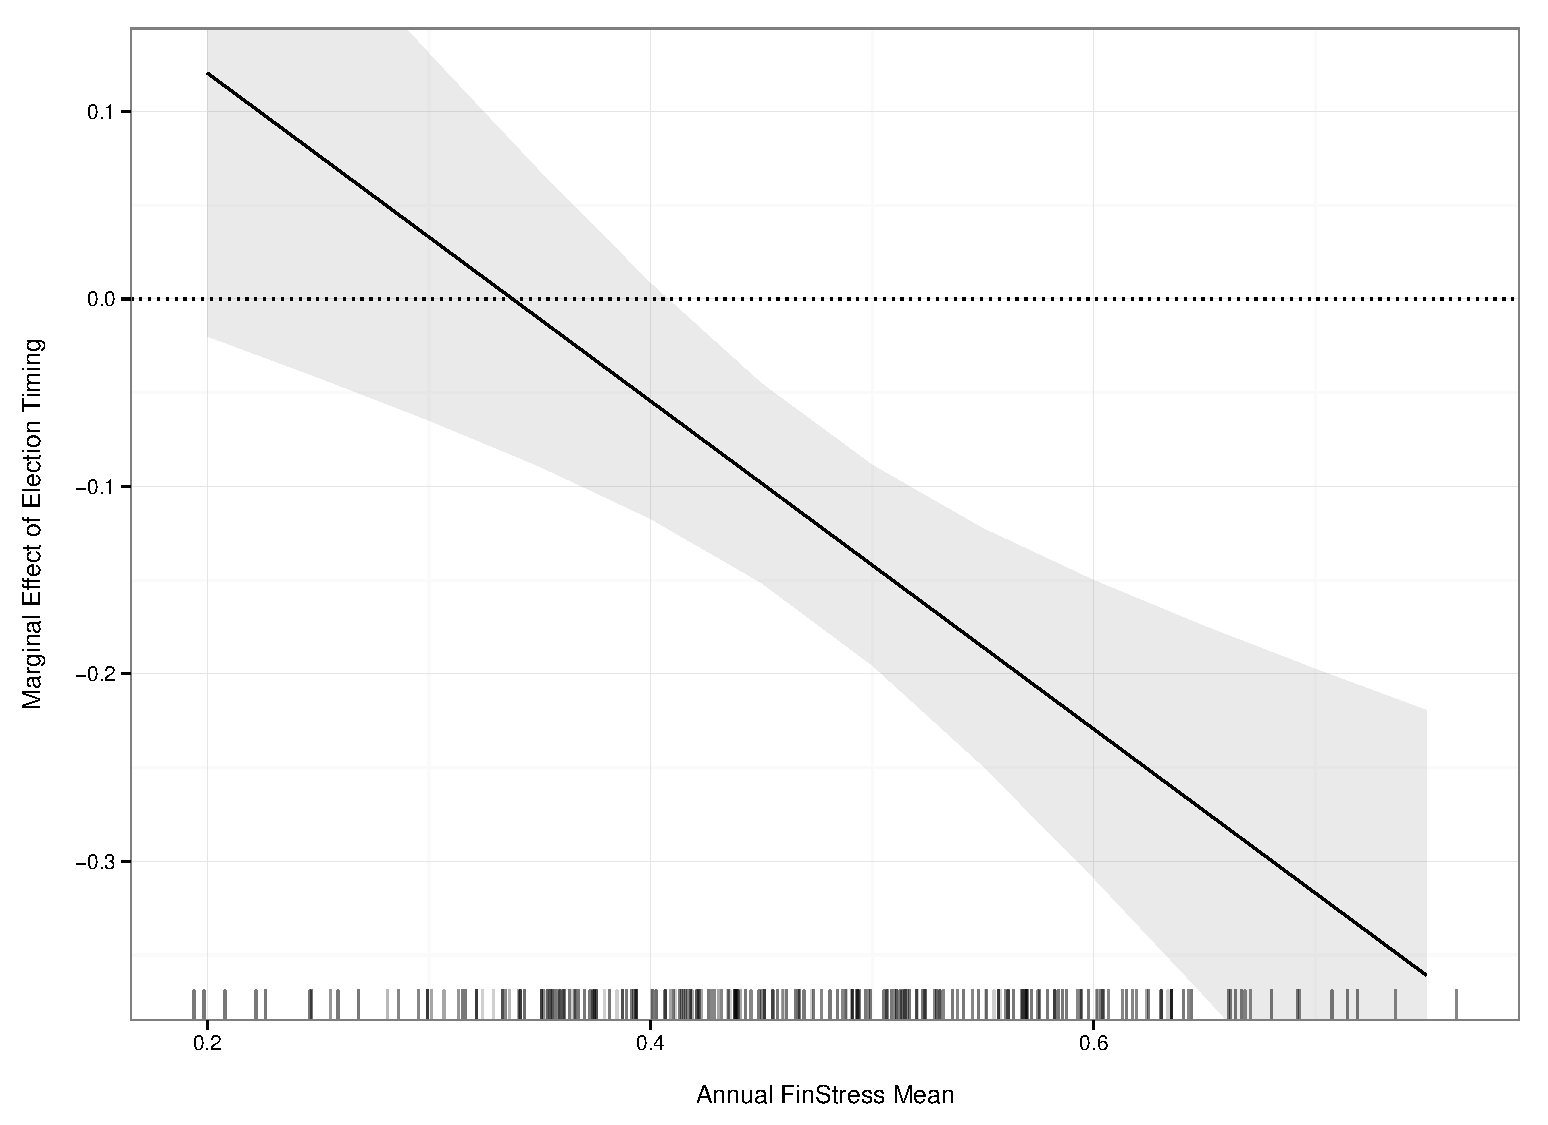
\includegraphics[scale=0.4]{figures/finstress_elect_me.pdf}
    \end{center}

\end{figure}

}

\frame{

\begin{figure}
    \caption{Marginal Effect of an Endogenous Election at Various Levels of Financial Market Stress on \textbf{Debt} Revisions}
    \label{me_finstress_endog_elect}

    \begin{center}
        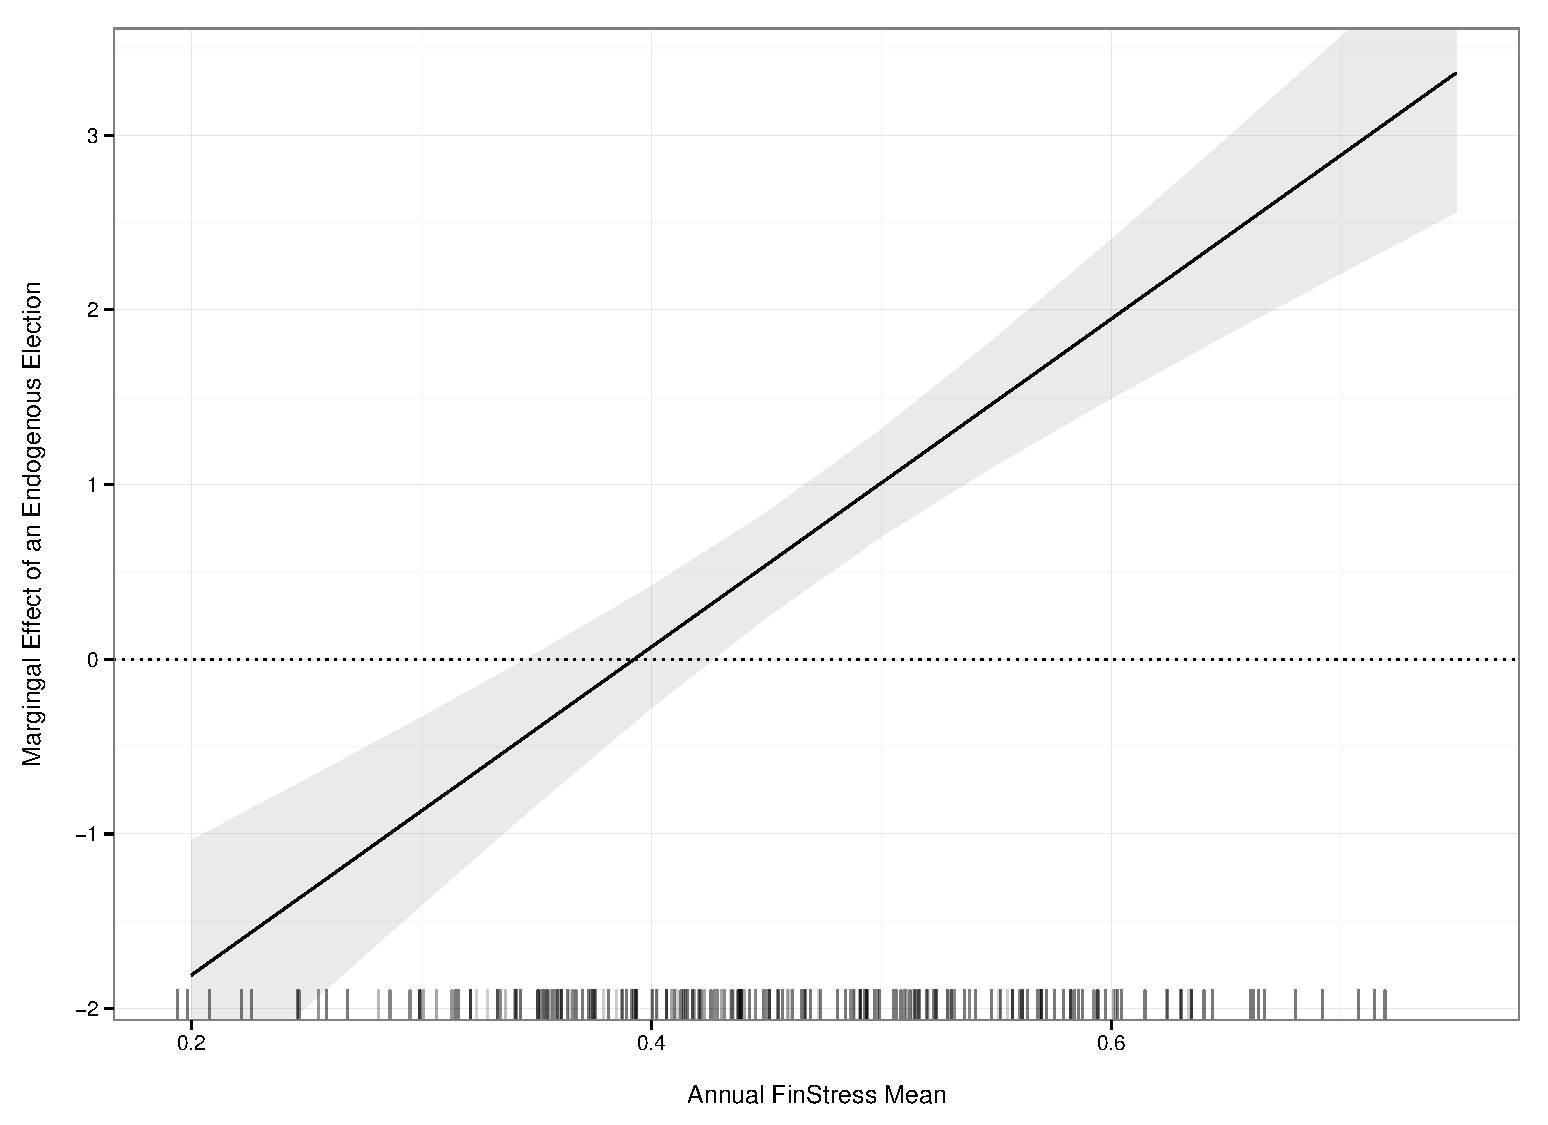
\includegraphics[scale=0.4]{figures/finstress_endog_elect_me.pdf}
    \end{center}

\end{figure}

}

\frame{

\begin{figure}
	\caption{Predicted \textbf{Debt} Revisions in Four Years After Publication for Years with Different Election Types/Non-election Years}
    \label{country_predict_debt_required}
    \begin{center}
    	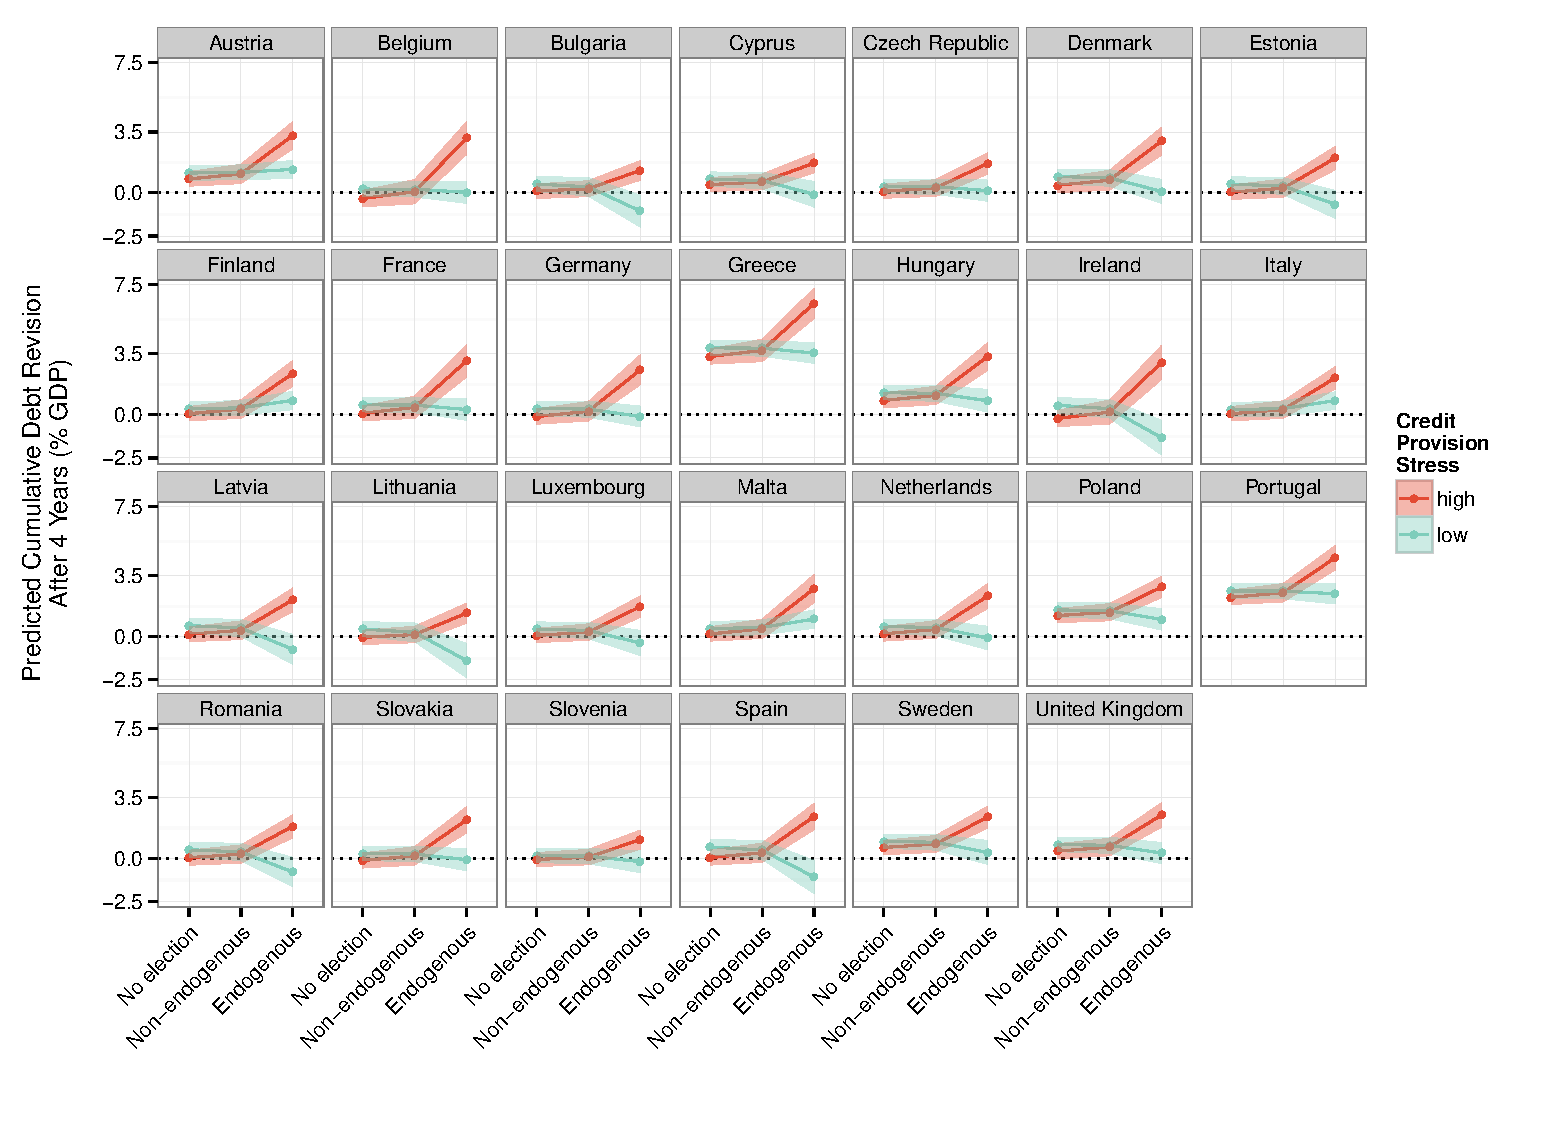
\includegraphics[scale=0.4]{figures/country_predict_required.pdf}
    \end{center}

\end{figure}

}

\frame{

\begin{figure}
    \caption{Marginal Effect of a Non-Endogenous Election at Various Levels of Financial Market Stress on \textbf{Deficit} Revisions}
    \label{me_finstress_non_endog_deficit}
    \begin{center}
        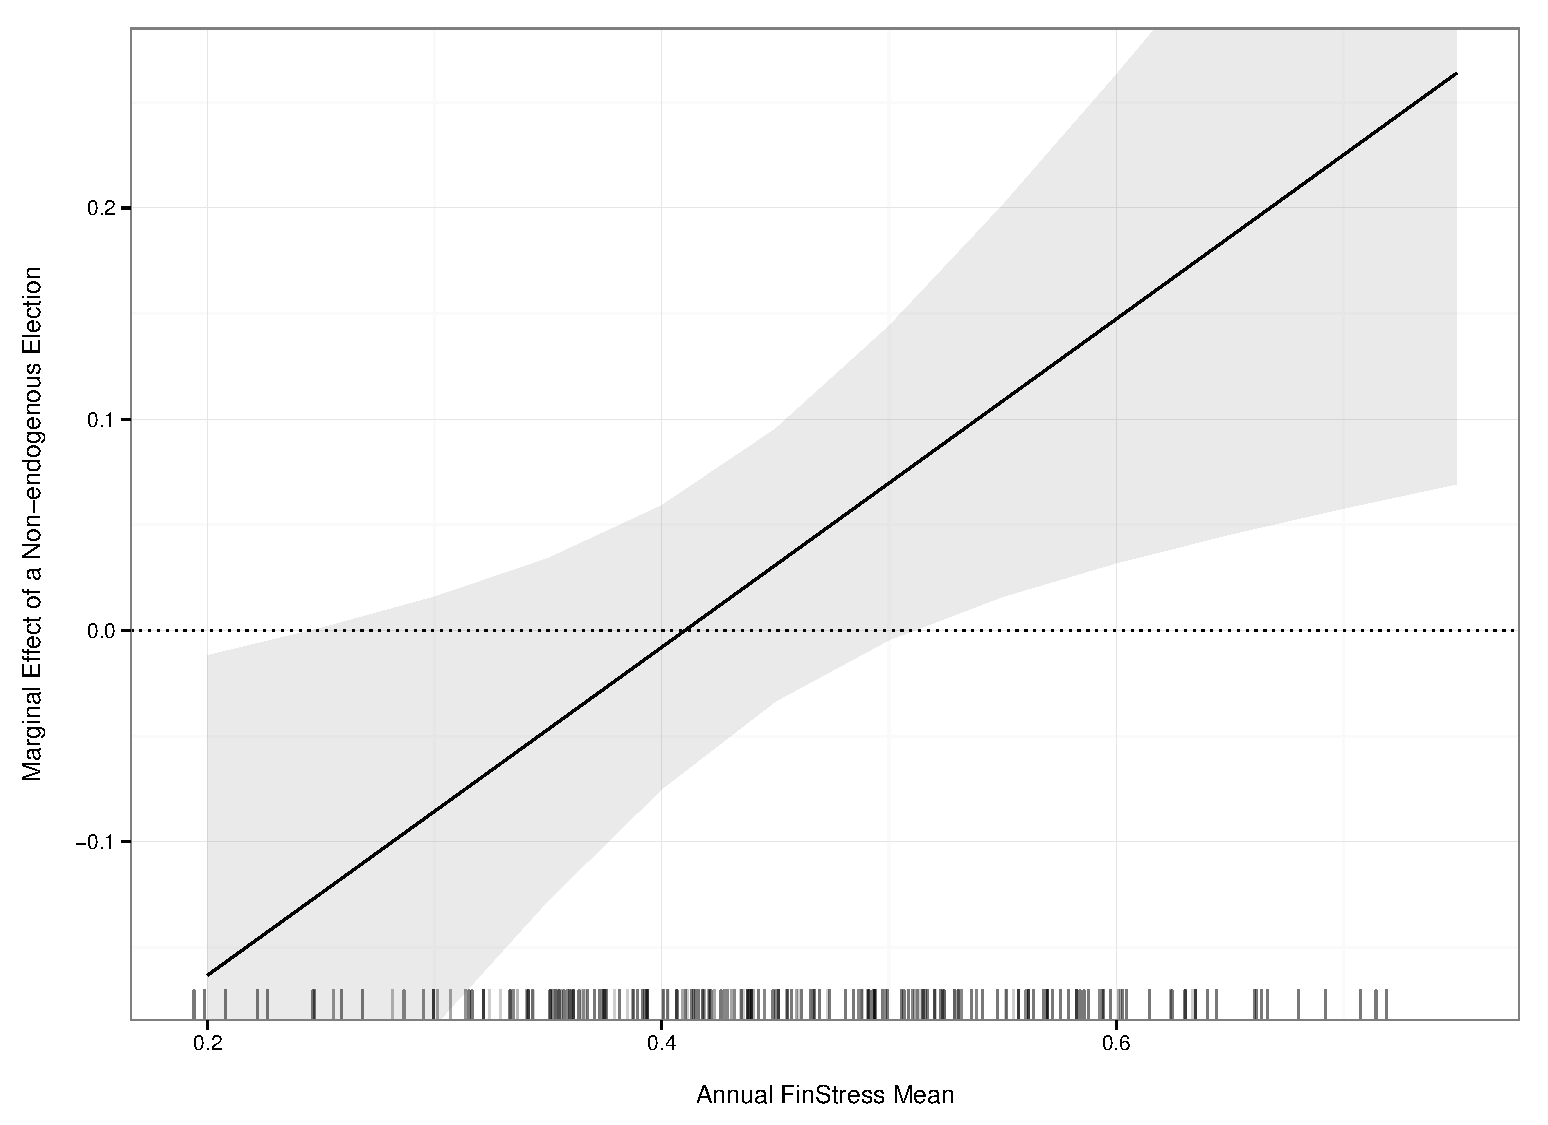
\includegraphics[scale=0.4]{figures/finstress_non_endog_deficit_me.pdf}
    \end{center}

\end{figure}

}


\section{Conclusion/Still to do}

\frame{
    \frametitle{To-Do}

    Omitted variables?:

    \begin{itemize}
        \item independence of national accounting agency.

        \item SGP enforcement actions (not just eurozone membership)

        \item Others?
    \end{itemize}

    \vspace{1cm}

    Model choice: normal linear regression with many 0s?

}

\end{document}
